\documentclass[11pt,]{article}
\usepackage[T1]{fontenc}
\usepackage{lmodern}
\usepackage{amssymb,amsmath}
\usepackage{ifxetex,ifluatex}
\usepackage{fixltx2e} % provides \textsubscript
% use upquote if available, for straight quotes in verbatim environments
\IfFileExists{upquote.sty}{\usepackage{upquote}}{}
\ifnum 0\ifxetex 1\fi\ifluatex 1\fi=0 % if pdftex
  \usepackage[utf8]{inputenc}
\else % if luatex or xelatex
  \ifxetex
    \usepackage{mathspec}
    \usepackage{xltxtra,xunicode}
  \else
    \usepackage{fontspec}
  \fi
  \defaultfontfeatures{Mapping=tex-text,Scale=MatchLowercase}
  \newcommand{\euro}{€}
\fi
% use microtype if available
\IfFileExists{microtype.sty}{\usepackage{microtype}}{}
\usepackage{graphicx}
% Redefine \includegraphics so that, unless explicit options are
% given, the image width will not exceed the width of the page.
% Images get their normal width if they fit onto the page, but
% are scaled down if they would overflow the margins.
\makeatletter
\def\ScaleIfNeeded{%
  \ifdim\Gin@nat@width>\linewidth
    \linewidth
  \else
    \Gin@nat@width
  \fi
}
\makeatother
\let\Oldincludegraphics\includegraphics
{%
 \catcode`\@=11\relax%
 \gdef\includegraphics{\@ifnextchar[{\Oldincludegraphics}{\Oldincludegraphics[width=\ScaleIfNeeded]}}%
}%
\ifxetex
  \usepackage[setpagesize=false, % page size defined by xetex
              unicode=false, % unicode breaks when used with xetex
              xetex]{hyperref}
\else
  \usepackage[unicode=true]{hyperref}
\fi
\hypersetup{breaklinks=true,
            bookmarks=true,
            pdfauthor={},
            pdftitle={},
            colorlinks=true,
            citecolor=blue,
            urlcolor=blue,
            linkcolor=magenta,
            pdfborder={0 0 0}}
\urlstyle{same}  % don't use monospace font for urls
\setlength{\parindent}{0pt}
\setlength{\parskip}{6pt plus 2pt minus 1pt}
\setlength{\emergencystretch}{3em}  % prevent overfull lines
\setcounter{secnumdepth}{0}
\usepackage{setspace}
%\singlespacing
\onehalfspacing
%\doublespacing
\setlength\parskip{0.11in}
\usepackage[vmargin=1.25in,hmargin=1.25in]{geometry}
%\usepackage{lineno}
%\linenumbers

\author{}
\date{}

\begin{document}

\section{I've submitted a paper. What happens
now?}\label{ive-submitted-a-paper.-what-happens-now}

Hurry up and wait. How long you'll have to wait largely depends on the
journal. Different journals have different steps in the editorial/review
process, and some are just inherently slower than others. The basic
process is summarised in the flow chart below, which comes from the
British Ecological Society's guide to peer review (worth reading,
especially if you're about to review a manuscript for the first time ---
the link is in the resources section). In addition to what's shown in
this figure, some especially high-impact journals (Nature and
Science\ldots{} perhaps others) also have ``Gatekeeper'' reviewers ---
who articles get sent to for a quick verdict on ``worth reviewing'' vs.
``reject without review'' before they actually go out for formal review.

\begin{figure}[htbp]
\centering
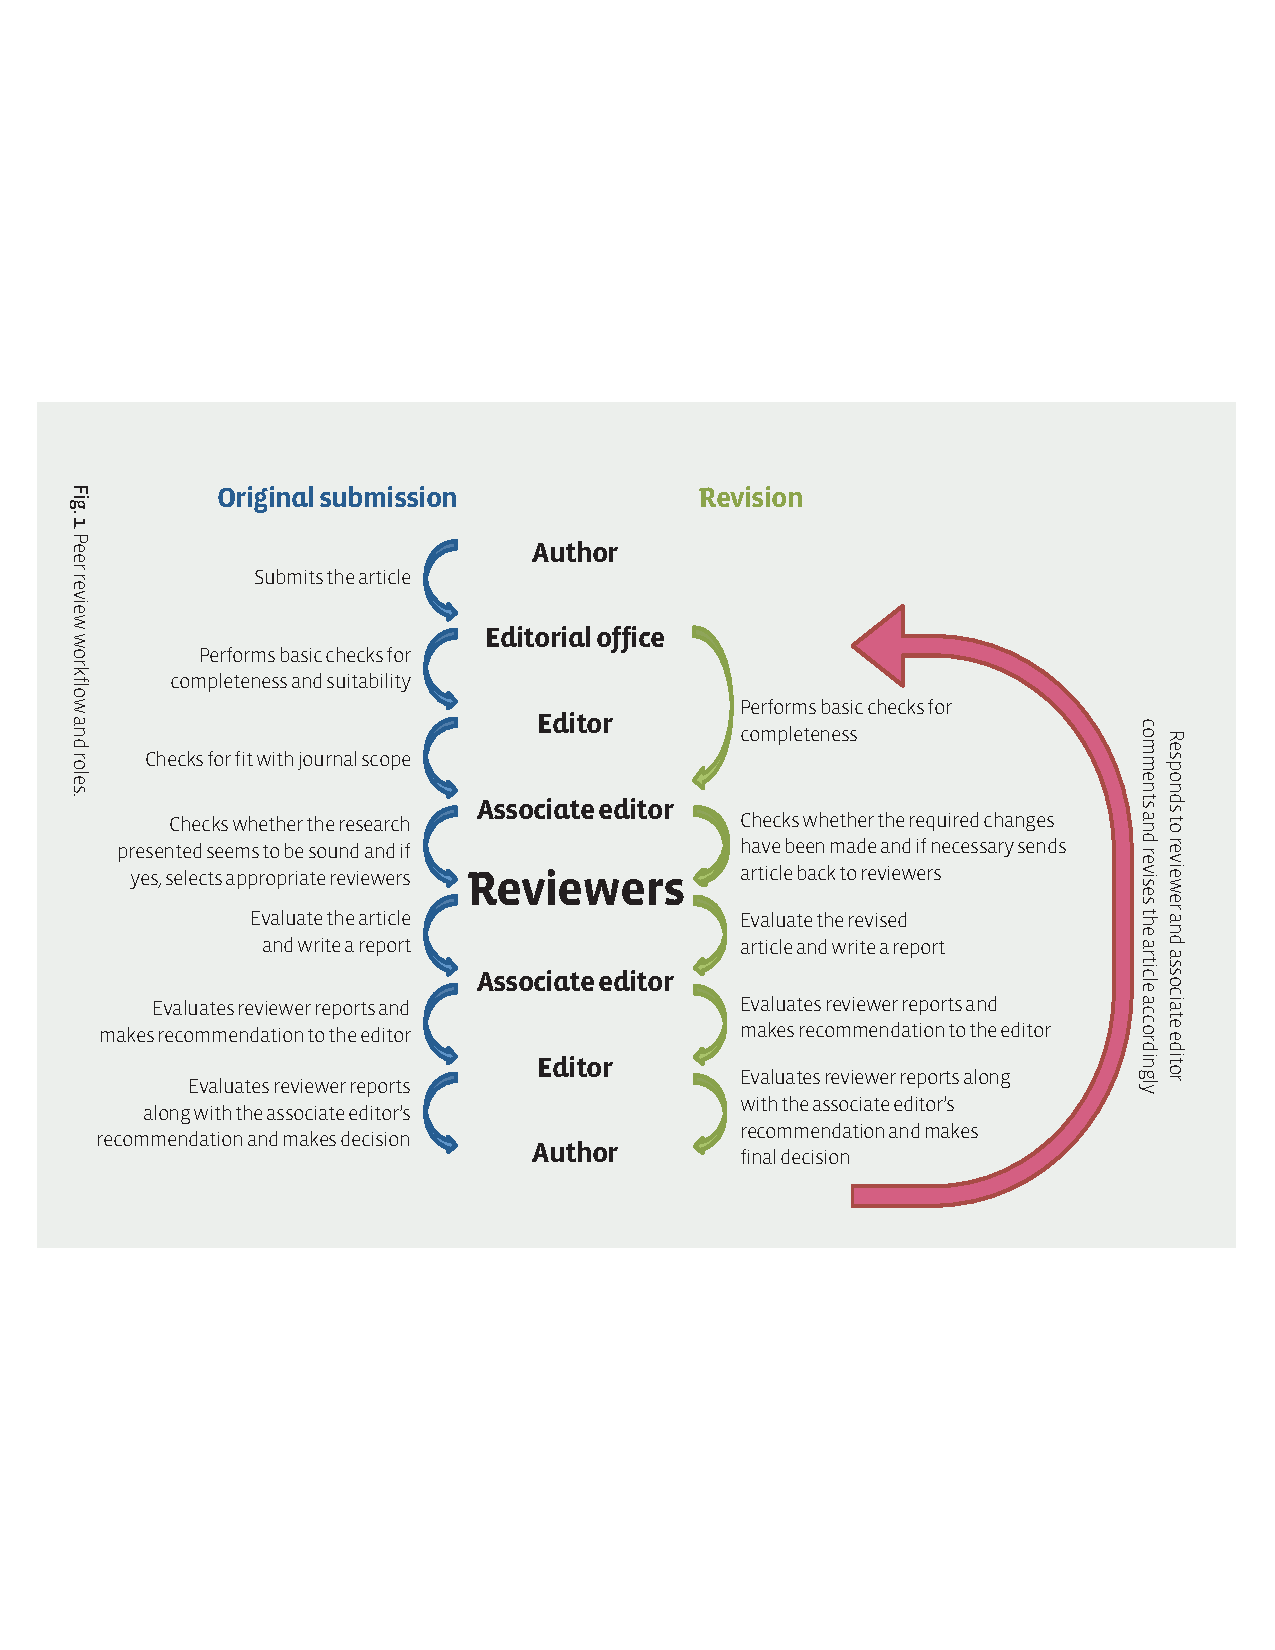
\includegraphics{BES_publishing_flowchart.pdf}
\caption{What happens to your paper after you submit it}
\end{figure}

What this boils down to is that, depending on the journal, you should
expect to hear back within anywhere from a few hours to a couple of
weeks, depending on whether your article has been sent out for review.
There are horror stories of people not hearing anything for 6 months,
only to be told that their MS wasn't even sent out for review, but this
definitely qualifies as a time when it's okay to bug the editor (see
below), and most of the time you should hear back pretty quickly.

Once your paper has been sent out for review, the fastest-turnaround
journals can have reviews back to you within a month. At the slowest
journals its not uncommon to wait several months.

Turn-around speed is something to weigh up pretty carefully when
submitting papers. Often there is a trade-off between publishing
somewhere high profile that might have a very slow turn-around,
vs.~somewhere a bit lower profile with a faster turn-around. Getting
papers out sooner can be important if you're applying for
jobs/scholarships etc., so its something to consider. Your supervisors,
peers, and other colleagues are your best resource for getting a handle
on the turn-around speed of a given journal. Journal websites often tell
you expected turn-around speed, but the estimates can be be (sometimes
wildly) optimistic. You can also check the submission, acceptance, and
publication dates on some recent articles if the journal publishes these
details. This is potentially biased though, as it's been suggested that
journals are increasingly giving ``reject with invitation to resubmit''
decisions rather than ``accept with major revisions'' to make their
submission to publication times appear shorter (see Dynamic Ecology
blog, link at bottom).

\subsection{When is it okay to bug the
editor?}\label{when-is-it-okay-to-bug-the-editor}

Sometimes. Its never a good idea to piss off the editor, but if you've
been waiting considerably longer than the estimated times provided by
the journal, \emph{politely} checking in about the status of your paper
is okay. Your advisor/senior collaborators are good people to ask if
you're unsure, and might even be willing to get in touch with the editor
on your behalf.

\subsection{Rejected?}\label{rejected}

Don't be disheartened. It's not necessarily a reflection on the quality
of your work. A surprising number of seminal papers were rejected on
their first submission. For example, Lindeman's paper that came up with
the concept of trophic levels got rejected when it was first submitted.
You'll probably end up with a better, more widely-read paper once you've
taken the reviewers' concerns on board.

An increasing number of journals now have ``trickle-down'' (or ``dumping
ground'', depending on your level of cynicism) sister journals. A couple
of examples are Ecosphere for Ecology and Ecosystems for Ecology
Letters, and there are many others. If the editor thinks your paper is
good but not quite sexy enough for the flagship journal, the rejection
may come with an invitation to ``transfer your submission'' or
``automatically resubmit'' to the sister journal.

If you get the option, transferring your submission to such a
``trickle-down'' journal can be a very convenient and time-effective way
to fast-track publication. Often your reviews carry over. The
disadvantage is that you may want to get the paper somewhere
higher-profile than the trickle-down option. In that case, you have to
figure out the trade-off of potential benefits vs.~the time cost and
risk of another rejection if you do resubmit.

If you do decide to resubmit elsewhere, \emph{implement suggested
changes you got from the first review}. You could well get the same
reviewers at the new journal and you don't want to piss them off! And
you'll probably end up with a better paper --- that's the point of peer
review.

\subsection{Not rejected}\label{not-rejected}

Yay! The 3 general ways in which your paper can be \emph{not} rejected
are:

\begin{enumerate}
\def\labelenumi{\arabic{enumi}.}
\itemsep1pt\parskip0pt\parsep0pt
\item
  Accepted with minor revisions.
\item
  Accepted with major revisions.
\item
  Invitation to revise and resubmit.
\end{enumerate}

Sometimes it may not be entirely clear from the Editor's letter which
category the decision falls into. A good rule of thumb is that if the
letter doesn't specifically mention the word ``rejected'', assume its 1
or 2. As mentioned above, option 3 is becoming increasingly common
(although some would argue that this decision should never happen in the
first place). The major difference in this case is that your paper may
still be rejected after re-submission so this can be a good time to
submit elsewhere if you feel it might be better received at another
journal.

\subsubsection{Responding to reviews}\label{responding-to-reviews}

The overall goal in responding to reviews is to convey the message: ``We
appreciate and acknowledge your criticism and advice; we understand your
misunderstanding; we have fully integrated your feedback'' (paraphrased
from the Matt Might blog post under Resources). In writing your response
letter

\textbf{Do:} Be polite, conciliatory and thorough. Do everything you can
to make the editors job as easy as possible.\newline{} \textbf{Don't:}
Tell the editor/reviewer that they don't know what they're talking
about, or totally ignore comments if you don't want to change something.

Your response will have two parts: your letter to the editor, and the
full response to reviewers. Its normally easier to do the full response
to reviewers first; the letter to the editor then summarises what you've
done. \bigskip{}

\emph{Documenting your revisions}

You should include \emph{everything} in your response, as you don't want
to give the impression that you are skipping anything. The best way make
sure you do this is to start by copying and pasting all the reviewer
comments into a new document and then interleaving your responses. Try
writing most or all of this before you actually implement changes. This
gives you a clear plan for the revisions, which can speed things up,
particularly if the reviewers have requested major changes. It also
helps you identify and figure out how you want to deal with any
potential conflicts between revisions the reviewers have requested.

Make this document as easy to navigate as possible. One way to do this
is to italicise all the reviewer comments, then indent your responses in
plain text below each point. Another way to do this is to structure the
document as a table with column headings something like:

\begin{tabular}{ | l | c | c | c | r | }
\hline
    Reviewer & Comment & Response & Section of paper\\
\hline
\end{tabular}

I haven't tried this method, but imagine it could get unwieldy if you
have numerous or complex revisions.

Usually reviewers will split their comments into ``major''
(e.g.~restructuring sections, concerns with methods or interpretations)
and ``minor'' (e.g. editorial changes). Its a good idea to deal with the
major comments up first.

Don't be surprised if the response ends up taking a LONG time to write,
and is a big document! But save yourself, the editor and the reviewers
time by using short one-word responses like ``Agreed.'' or ``Amended.''
where appropriate.

\bigskip{}

\emph{The letter to the editor}

The letter to the editor gives an succinct overview of your revisions.
Making this summary clear and concise is particularly important if the
full response is long. The letter should almost always include something
along the lines of:

\begin{quote}
``We have addressed all the reviewers concerns and implemented their
suggested changes, and in doing so our manuscript has been greatly
improved. We have provided a detailed description of specific changes in
our response to the reviewers comments (see attached document).''
\end{quote}

In the letter, you can make comments to the editor that the reviewers
won't see. So, If you think the reviewers are were totally out to lunch
with some or all of their comments, the letter is where you should
highlight this to the editor. You can even make the decision to write to
the editor rebutting the reviews rather than addressing the suggestions
--- but you need to be really sure of yourself to do this, and your
chances of success are low. Pick your battles. \bigskip{}

\emph{Other points to bear in mind when making revisions:}

\begin{itemize}
\itemsep1pt\parskip0pt\parsep0pt
\item
  Remember that the reviewers volunteered to offer you comments to
  improve your work --- always take a tone of thankfullness in your
  response. Make sure to get across that you're thankful for the
  reviewer's suggestions and emphasize how the changes have improved the
  manuscript.
\item
  Be clever about your wording if there are things you don't want to
  change. Sentences like ``We can see that our wording was unclear and
  we have rewritten lines xxx to yyy to improve clarity. We hope this
  alleviates the reviewer's concerns.'' can work well.
\item
  If the reviewers didn't criticize it, think \emph{very} carefully
  before touching it; you don't want to create new content that the
  editor feels needs to be peer reviewed.
\item
  If you edited the paper in any way besides in response to the
  reviewers, note it to the editor.
\item
  Many journals will request a tracked-changes version, some that don't
  will still appreciate it, some will specifically say not to. Do
  whatever is requested.
\item
  Pick your battles wisely\ldots{} you can sometimes push back on a
  limited number of reviewer requests, but for the most part you need to
  just do it. If you're indifferent one way or other, just do it so you
  can push back where you feel it is important. \bigskip{}
\end{itemize}

\subsection{Resources}\label{resources}

\emph{These are hyperlinks in the electronic version of this handout;
you should be able to find the relevant links easilily on Google, though
}

\begin{enumerate}
\def\labelenumi{\arabic{enumi}.}
\itemsep1pt\parskip0pt\parsep0pt
\item
  \href{http://www.britishecologicalsociety.org/wp-content/uploads/Publ_Peer-Review-Booklet.pdf}{BES
  guide to Peer Review in Ecology and Evolution}
\item
  \href{https://www.google.com/url?sa=t\&rct=j\&q=\&esrc=s\&source=web\&cd=1\&cad=rja\&uact=8\&ved=0CCgQFjAA\&url=http\%3A\%2F\%2Fwww.griffith.edu.au\%2F__data\%2Fassets\%2Fpdf_file\%2F0007\%2F435526\%2FWriting-Ecology-Research-Papers-July-2012.pdf\&ei=QHAzU97cL4XtoASU44DwBQ\&usg=AFQjCNETmGdH64aWIK9cdKO-g2i9LTl2nA\&sig2=bNmGEzkhR8Ucz_pzrd1uAQ\&bvm=bv.63808443,d.cGU}{Griffith
  University guide on How to write Ecology Research Papers}
\item
  \href{http://conservationbytes.com/2012/10/22/how-to-write-a-scientific-paper/}{Conservation
  Bytes Blog on writing papers}
\item
  \href{http://matt.might.net/articles/peer-review-rebuttals}{Matt Might
  blog post on how to write rebuttals to reviewer comments}
\item
  \href{http://dynamicecology.wordpress.com/2014/03/12/tell-me-again-what-major-revisions-are/}{Dynamic
  Ecology Blog post on interpreting Editors' decisions} 
\end{enumerate}

\emph{Prepared by Rowan Trebilco as a handout for SFU Grad Caucus
Publishing workshop, 2014. Sean Anderson provided useful comments and
suggestions on an earlier draft.}

\end{document}
